\documentclass[../../main.tex]{subfiles}

% 

\begin{document}
\chapter{Teorie jaderných procesů}

\section{Zadanie}

Energie reakce, Energie rozpadu, Výtěžek jaderných reakcí(tlustý a tenký terčík), Zákony zachování, Princip detailní rovnováhy, Klasifikace jaderných reakcí, Mechanismy jaderných reakcí(model složeného jádra, přímé reakce, optický model atomového jádra), Štěpení, Syntéza, Uvést příklady některých důležitých jaderných reakcí.

\section{Historický přehled studia jaderných reakcí}

Termín jaderná reakce je značně široký, ve fyzice atomového jádra si pod ním představujeme interakci nebo jinak řečeno srážku dvou mikročástic, ze které se opět vynořují mikročástice. Alespoň jedna z těchto mikročástic musí být jádrem s atomovým číslem $Z$ větším než jedna. Jaderné reakce probíhají v podstatě v neomezeném intervalu energií, ve fyzice atomového jádra však máme na mysli relativní kinetické energie převážně v intervalu od nuly do 100 $\mathrm{MeV}$, výjimečně až do hodnot rovných řádově několika $\mathrm{GeV}$. 

\begin{itemize}
	\item r. 1919 - Ernest Rutherford - 1. umělá jaderná reakce $\alpha + ^{14}_{7}N \rightarrow ^{17}_{8}O + p$
	\item r. 1924 $\rightarrow$ potvrzeno Blackettem za použití Wilsonovy mlžné komory
	\item r. 1932 - objev neutronu J. Chadwickem v reakci $\alpha + ^{9}_{4}Be \rightarrow ^{12}_{6}C + n$
	\item r. 1932 - Cockroft a Walton $\rightarrow$ 1. reakce s urychlenými protony: $p + ^{7}_{3}Li \rightarrow 2 \alpha$
	\item v r. 1934 - manželé Curierovi objevili umělou radioaktivitu
	\item v r. 1939 - objeveno štěpení uranu $\rightarrow$ Hahn, Strassmann
	\item v r. 1942 $\rightarrow$ Fermi - spuštění 1. jaderného reaktoru s přírodním uranem o výkonu několika wattů
	\item r. 1951 $\rightarrow$ 1. jaderná ponorka (Nautilus)
	\item r. 1955 $\rightarrow$ 1. jaderná elektrárna (Snipping Port)	
\end{itemize} 

\section{Základní pojmy}

- zapisujeme jako relaci tak, že na levé straně se píšou objekty vstupující do reakce a na pravé straně objekty z ní vystupující, od vstupujících k vystupujícím směruje šipka definující, které objekty považujeme za počáteční a které za koncové

$\rightarrow$ sevřený zápis $\Rightarrow$ jen tehdy, když v reakcích vystupují elementární částice nebo jádra helia ($\alpha$), deuteronu (d), tritia (t) $\Rightarrow$ odpovídá experimentu $\Rightarrow$ těžké částice vstupující do reakce  jsou zpravidla nehybným terčíkem, lehká částice je obvykle na jistou energii urychleným projektilem

- Zápis: $a + A \rightarrow C^* \rightarrow B + b$, ~~~~~~ $C^*$... složené jádro, mezistav, přes který může reakce probíhat

- Sevřený zápis: $A(a,b)B$

\subsection{Různé procesy}
\begin{itemize}
	\item $\rightarrow$ pružný rozptyl $(n,n), (p,p)$
	\item $\rightarrow$ nepružný rozptyl $(n,n^{'}), (p, p^{'}),...$
	\item $\rightarrow$ jaderné reakce: 
	\begin{itemize}
		\item $\rightarrow$ vznik nového jádra a částice - $A(a,b)B$
		\item $\rightarrow$ vznik nového jádra a více částic - $A(a,b_1 b_2 b_3....)B$
		\item $\rightarrow$ štěpení jádra - $(n,f)$
		\item $\rightarrow$ tříštění jader
	\end{itemize}
\end{itemize}

\subsection{Základní definice}
\begin{itemize}
	\item vstupní kanál - částice (jádra) a jejich charakteristiky (energie, hybnosti, spiny, ....) do reakce vstupující
	\item výstupní kanál - částice (jádra) a jejich charakteristiky z reakce vystupující
	\item účinný průřez $\sigma$ - závisí na energiích, hybnostech, spinech, nábojích $\Rightarrow$ pravděpodobnost, že při srážce $A+a$ dojde k přeměně $a+A \rightarrow b+B$ , $[\sigma] = \mathrm{m^2}$
	\item excitační funkce - závislost účinného průřezu na energii $\sigma (E)$ - excitační funkce
	\item prahová reakce - nastávají až od určité energie
	\item výtěžek reakce - počet přeměn dělený počtem nalétávajících částic
	\item tenký terčík - nezmění hustotu a energii částic svazku
	\item tlustý terčík - hustota a energie částic svazku se mění
\end{itemize}

\subsection{Zákony zachování}

$\Rightarrow$ energie, hybnosti, momentu hybnosti, el. náboje, parity, baryonového a leptonového čísla

\begin{itemize}
	\item Energie a hybnosti 
	\begin{itemize}
		\item lze určit směry výletu a možné energie produktů reakce
		\item pro určení úhlového rozdělení a energetického rozdělení je třeba znát typ interakce
		\item k nalezení možných směrů výletu produktů reakce lze použít vektorový diagram hybností $\Rightarrow$ diagram nezávisí na typu interakce a lze jej použít pouze pro nerelativistické přiblížení
	\end{itemize}
	\item Momentu hybnosti
	\begin{itemize}
		\item pouze diskrétní hodnoty $l =0,1,2,3,....$ ~~~~~~ $[\hbar]$
		\item pro nízké energie a krátký dosah sil $\rightarrow$ reakce možná pouze pro ohraničené nevelké číslo $l$
		
		$\Rightarrow$ výhodné přejít do vlastních stavů momentu hybnosti
		\item poloklasicky  $p b =l \hbar$ $\Rightarrow$ $l \leq \dfrac{p b_{max}}{\hbar} = \dfrac{2 \pi R}{\lambda}$ 
	\end{itemize}
	\item Náboje - suma el. nábojů před reakcí a po ní se zachovává
	\item Baryonového čísla - pro nízké energie ($E < m_n c^2$) $\rightarrow$ zákon zachování  počtu nukleonů
	\item Parity - parita výchozího stavu se během reakce nemění, protože při změně relativního orbitálního momentu $\Pi_f = (-1)^{\Delta l}\Pi_i$, např. při pružném rozptylu, nemůže dojít ke změně orbitálního momentu o $\Delta l =$ liché, i když by to při změně orientace spinu bylo z hlediska zachování momentu hybnosti možné
	
	\item REAKCE POD VLIVEM SILNÉ INTERAKCE - platí zákon zachování celkového izotopického spinu (izospin) i zákon zachování jeho projekce do jedné ze souřadných os a dále zákon zachování parity
	\item REAKCE POD VLIVEM ELEKTROMAGNETICKÉ INTERAKCE - neplatí zákon zachování celkového izotopického spinu
	\item REAKCE POD VLIVEM SLABÉ INTERAKCE - neplatí zákon zachování izospinu v žádné formě, ani zákon zachování parity
\end{itemize}

\section{Energie reakce, energie rozpadu}
\begin{itemize}
	\item Energie reakce $Q$: rozdíl sumy klidových energií částic před reakcí a po ní nebo jako rozdíl sumy kinetických reakcí po reakci a před ní:
	\begin{equation}
	Q = \sum_{j=1}^{n_i}m_j c^2 - \sum_{k=1}^{n_f} m_k c^2 = \sum_{k=1}^{n_f} T_K - \sum_{j=1}^{n_i} T_j
	\end{equation}
	$\Rightarrow$ $Q$ nezávisí na souřadné soustavě
	
	$\Rightarrow$ 3 druhy reakcí: 
	\begin{itemize}
		\item Exoergická reakce: $Q>0$ $\Rightarrow$ energie se uvolňuje (samovolné rozpady jader či částic, reakce probíhající při libovolné energii nalétávající částice). V případě rozpadu hovoříme o energii rozpadu.
		\item Pružný rozptyl: $Q=0$
		\item Endoergická reakce: $Q<0$ $\Rightarrow$ existuje práh reakce, energii je třeba dodat, aby se reakce vůbec uskutečnila
	\end{itemize}
	
- zůstane-li jádro B ve vzbuzeném stavu $\Rightarrow$ $Q - E^* = T_b + T_B - T_a - T_A$, kde $E^*$ je excitační energie	
\end{itemize}

\subsection{Prahová energie}

- v těžišťové souřadné soustavě (CMS):
\begin{itemize}
	\item počáteční stav: $\sum_{j=1}^{n_i} \vec{p_j}' = 0$
	\item ZZH (konečný stav): $\sum_{k=1}^{n_f} \vec{p_k}' = 0$
	\item reakce může nastat, pokud $\sum_{k=1}^{n_f} T_k ^{'} \geq 0$
	\item prahová energie v CMS 
	\begin{equation}
	T_{THR}^{'} = - Q = \sum_{k=1}^{n_i}T_{k}^{'} = \sum_{k=1}^{n_f} m_k c^2 - \sum_{j=1}^{n_i} m_j c^2 = |Q|
	\end{equation}
\end{itemize}

- prahová energie v LAB pro projektil a terčík ($p_2 = 0$)
\begin{itemize}
	\item kinetická energie těžiště ($T = p^2 /2m$)
     \begin{equation}
     T_{CMS} = \dfrac{p_{1}^{2}}{2(m_1 + m_2)}
     \end{equation}
     \begin{equation}
     T_{THR} = T_i = |Q| \left( 1 + \dfrac{m_1}{m_2}\right) 
     \end{equation}
\end{itemize}

\begin{center}
	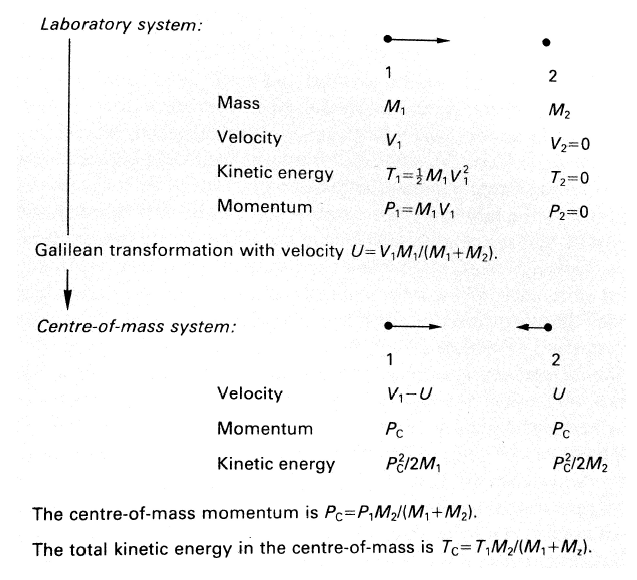
\includegraphics[width=0.6\textwidth]{soustava.png}
	\captionof{figure}{Srovnání laboratorní a těžišťové soustavy}		
\end{center}

\subsection{Srážkový diagram hybností}
- Předpokládáme, že terčové jádro je v klidu

- Vztahy mezi hybnostmi částic před a po srážce:
\begin{equation}
v_{1}' = \tilde{v_{1}}' + v_{CM} , ~~~~~~ p_{1}' = \tilde{p_{1}}' + \dfrac{m_1}{m_1 + m_2} p_1
\end{equation}
\begin{equation}
v_{2}' = \tilde{v_{2}}' + v_{CM}, ~~~~~~ p_{2}' = - \tilde{p_{1}}' + \dfrac{m_2}{m_1 + m_2} p_1
\end{equation}


\begin{table}[h]
\centering
\caption{Přehled hybností}
\begin{tabular}{|c|c|c|c|c|}
\hline
 & \multicolumn{2}{|c|}{Před zrážkou} & \multicolumn{2}{|c|}{Po zrážce} \\ \hline
 & LAB & CMS & LAB & CMS \\ \hline
Částice 1 & $p_1$ & $\tilde{p_1}=p_1\frac{m_2}{m_1+m_2}$ & $p_1'=\tilde{p_{1}}' + \frac{m_1}{m_1 + m_2} p_1$ & $\tilde{p_1}'$ \\ \hline
Částice 2 & $p_2=0$ & $\tilde{p_2}=-p_1\frac{m_2}{m_1+m_2}$ & $p_2'=- \tilde{p_{1}}' + \frac{m_2}{m_1 + m_2} p_1$ & $\tilde{p_2}'=-\tilde{p_1}'$ \\ \hline
\end{tabular}
\end{table}

Sečteme-li tyto rovnice, dostaneme zákon zachování hybnosti pro zkoumaný případ: $p_{1} = p_{1}' + p_{2}'$

- Konstrukce vektorového diagramu hybností:
\begin{itemize}
	\item hybnost $p_1$ dopadající částice zobrazíme orientovanou úsečkou $AC$
	\item rozdělíme úsečku $AC$ na dvě části v poměru $AO:OC = m_1:m_2$
	\item kolem bodu 0 opíšeme kružnici procházející bodem $C$ $\Rightarrow$ její poloměr je roven velikosti hybnosti $p_1$ v těžišťové soustavě $\tilde{p_{1}} = \dfrac{m_2}{m_1 + m_2} p_1$
	
	$\Rightarrow$ kružnice je geometrickým místem vrcholů $B$ vektorového trojúhelníku hybností $ABC$ (znázorňuje zákon zachování hybnosti), jehož strany $AB$ a $BC$ představují možné hybnosti částic po srážce v laboratorní soustavě. 

\end{itemize}

\begin{figure}[h!]
	\centering
	\begin{subfigure}[c]{0.3\textwidth}
		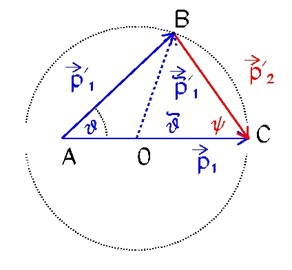
\includegraphics[width=\linewidth]{diag1.jpg}
		\caption{$m_1 < m_2$}
	\end{subfigure}
	\hfill
	\begin{subfigure}[c]{0.3\textwidth}
		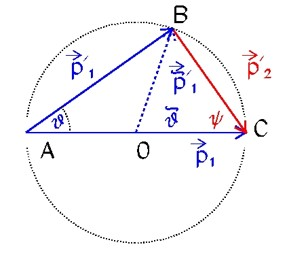
\includegraphics[width=\linewidth]{diag2.jpg}
		\caption{$m_1 = m_2$}
	\end{subfigure}
	\hfill
	\begin{subfigure}[c]{0.3\textwidth}
		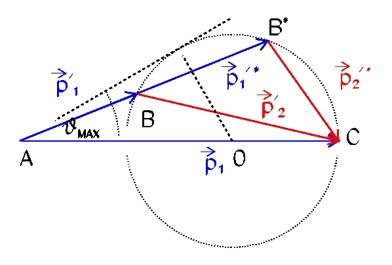
\includegraphics[width=\linewidth]{diag3.jpg}
		\caption{$m_1 > m_2$}
	\end{subfigure}
	\caption{Konstrukce vektorového diagramu hybností}
\end{figure}


V závislosti na poměru hmotností částic se může bod $A$ nacházet uvnitř dané kružnice, na ní nebo 
vně. Úhel rozptylu v těžišťové soustavě může nabývat všechny možné hodnoty  $\tilde{\vartheta}$ od $0$ do $\pi$. Dovolené hodnoty úhlu rozptylu $\vartheta$ v laboratorní soustavě a úhlu odrazu $\psi$ v laboratorní soustavě jsou v tabulce: 

\begin{figure}
	\centering
	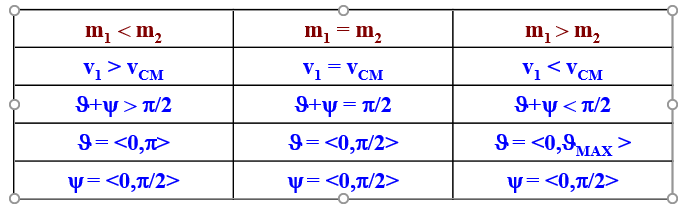
\includegraphics[width=1\textwidth]{srazkovy.png}
	\caption{Dovolené hodnoty úhlu rozptylu $\vartheta$ v laboratorní soustavě a úhlu odrazu $\psi$ v laboratorní soustavě}		
\end{figure}
\begin{figure}
	\centering
	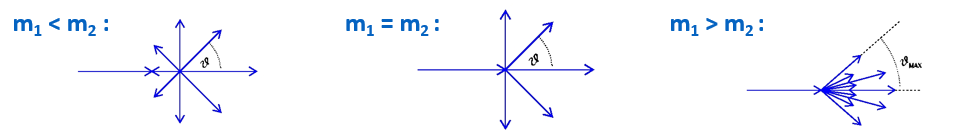
\includegraphics[width=1\textwidth]{srazkovy2.png}
	\captionof{figure}{Dovolené hodnoty úhlu rozptylu $\vartheta$ v laboratorní soustavě }		
\end{figure}

V laboratorní soustavě: 
\begin{itemize}
	\item $m_1 < m_2$ $\rightarrow$ dopadající částice rozptýleny do obou polokoulí
	\item $m_1 = m_2$ $\rightarrow$ dopadající částice rozptýleny do přední polokoule
	\item $m_1 > m_2$ $\rightarrow$ dopadající částice rozptýleny do přední polokoule do kužele s vrcholovým úhlem $2 \vartheta_{max}$ (osou kužele je směr dopadajících částic): $ \sin \vartheta_{max} = m_2 /m_1$	 
\end{itemize}

Vztah mezi úhly rozptylu a odrazu v laboratorní a těžišťové soustavě (připomínka předpokladu pružného rozptylu):
\begin{equation}
\psi = \dfrac{\pi - \tilde{\vartheta}}{2}   ~~~~~~~~ \tan \vartheta = \dfrac{\sin \tilde{\vartheta}}{\cos \tilde{\vartheta} + (m_1 / m_2 )}.
\end{equation}

Vektorový diagram hybností poskytuje veškerou informaci, kterou lze získat z pouhých zákonů zachování hybností a energií. Ukazuje možné varianty rozletu částic, nic ale neříká o pravděpodobnostech realizace jednotlivých možných variant. 

\section{Výtěžky reakcí, účinný průřez}
\begin{itemize}
	\item ÚČINNÝ PRŮŘEZ - $\sigma$ $\Rightarrow$ pravděpodobnost, že při srážce $a + A$ dojde k přeměně $a+A \rightarrow B+b$
	
	$\Rightarrow$ závisí pouze na typu interakce (slabá, silná, elektromag.) mezi $a$ a $A$, základních charakteristikách $a$ a $A$ a pohybových vlastnostech $a$ a $A$
	
	$\Rightarrow$ nezávisí na hustotě toku dopadajících částic typu $a$, ani na počtu ostřelovaných terčových jader typu $A$ $\Rightarrow$ nezávisí na provedení experimentu
	
	\item VÝTĚŽEK - $\omega$ $\Rightarrow$ udává podíl počtu přeměn $\Delta N$ na počtu dopadajících částic $N_0$
	\begin{equation}
	\omega = \dfrac{\Delta N }{N_0}
	\end{equation}
	$\Rightarrow$ bezrozměrná veličina
	
	$\Rightarrow$ závisí na účinném průřezu $\sigma$, na kinetické energii nalétávající částice $T_a$ a na konkrétním terčíku, proto nemůže sloužit jako univerzální charakteristika jaderné reakce
	
	$\Rightarrow$ závisí na tom, zda je terčík tenký nebo tlustý
	
	\item TENKÝ TERČÍK $\Rightarrow$ nemění energii a hustotu částic svazku
	
	$\Rightarrow$ na všechna terčíková jádra dopadá stejný tok $N_0$ ostřelujících částic téže energie (všechny terčové částice mají stejnou šanci zúčastnit se jaderné reakce)
	
	$\Rightarrow$ počet částic $N_0$ se nemění s hloubkou terče, stejně jako jejich kinetická energie $T_a$
	
	$\Rightarrow$ výtěžek:
	\begin{equation} 
	\omega = \dfrac{\Delta N }{N_0} = \sigma \cdotp  n \cdotp x << 1,
	\end{equation}
	kde $\sigma$ je celkový účinný průřez, $n$ je počet terčíkových jader v 1 $\mathrm{m^3}$ a $x$ je tloušťka terče $\Rightarrow$ $n \cdotp x$ je plošná hustota terče.
	
	\item TLUSTÝ TERČÍK $\Rightarrow$ hustota a energie částic svazku se mění $\Rightarrow$ průběh závisí na tom, o jaký typ částic jde 
	\begin{itemize}
		\item reakce s nabitými částicemi
		\item reakce s neutrony 
		\item reakce s fotony
	\end{itemize}
\end{itemize}

\subsection{Interakce v terčíku}

\begin{center}
	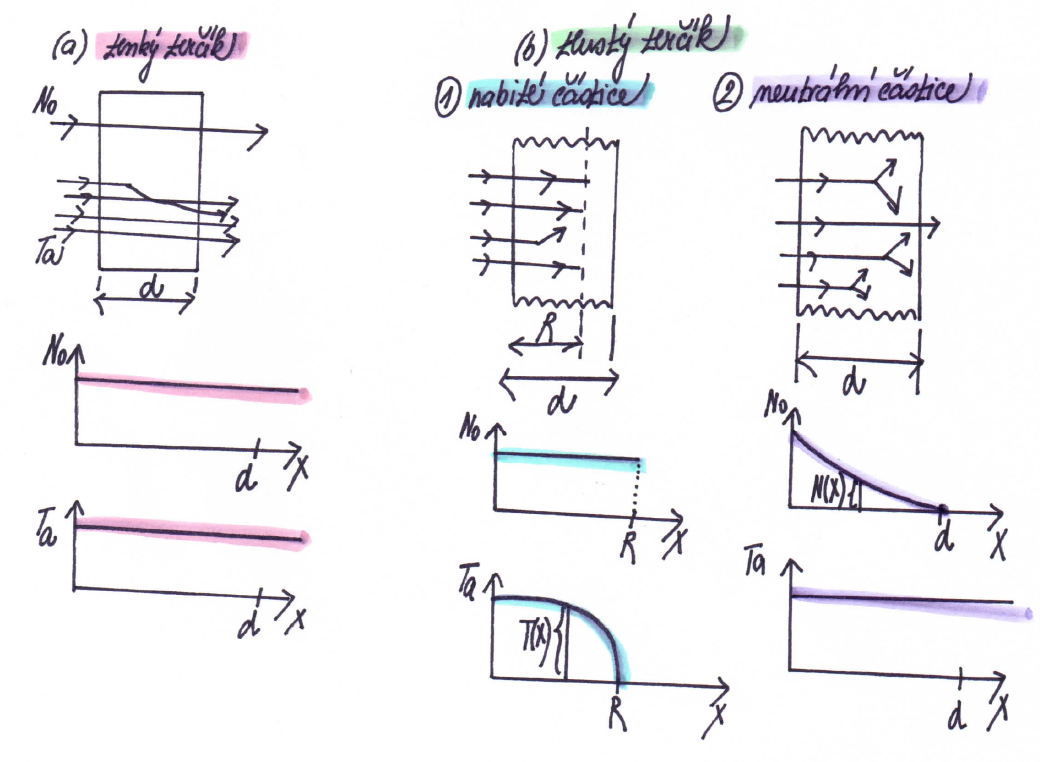
\includegraphics[width=1\textwidth]{terc.png}
	\captionof{figure}{Interakce v terčíku}		
\end{center}
	
\section{Reakce s nabitými částicemi}

- ztráta energie ionizací a excitací terčíkových atomů

- reakce nastávají při různé energii $T$ nalétávajících částic: $\sigma(T)$

- celkový počet částic se mění jadernými reakcemi $\Rightarrow$ lze zanedbat $N(x) = N_0$

- tlustý terč (tloušťka $d$ $>$ dolet $R$)
\begin{equation}
dN = N(x) \cdotp n \cdotp \sigma(x) \cdotp dx \cong N_0 \cdotp n \cdotp \sigma(x) \cdotp dx
\end{equation}

- výtěžek reakce je (při $d > R$)
\begin{equation}
\omega = \dfrac{\Delta N}{N_0 } = n \cdotp \int_{0}^{R} \sigma(x) dx = n \cdotp \int_{T_a}^{0} \dfrac{\sigma(T)}{\dfrac{dT}{dx}} dT = n \int_{0}^{T_a} \dfrac{\sigma(T)}{- \dfrac{dT}{dx}} dT
\end{equation}

z $-\dfrac{dT}{dx}$ $\Rightarrow$ vyšší $T_a$, $\sigma(T)$ a nižší energetické ztráty $\Rightarrow$ vyšší dolet a výtěžek $\omega = \omega (T)$ - excitační funkce

$\Rightarrow$ 
\begin{equation}
\sigma(T) = \dfrac{1}{n} \dfrac{d \omega}{dT} \left| \dfrac{dT}{dx} \right| 
\end{equation}

- střední účinný průřez 
\begin{equation}
\bar{\sigma} = \dfrac{1}{R} \int_{0}^{R} \sigma(x) dx \Rightarrow \omega = n \cdotp \bar{\sigma } \cdotp R
\end{equation}

\section{Reakce s neutrony}

- neinteragují s atomovými obaly, pouze rozptyl a absorbce na jádrech

- ubývá počet neutronů, ale jejich energie se příliš nemění

- svazek monoenergetických neutronů o hustotě toku $N_0$

- počet reakcí $dN$ ve vrstvě terče $dx$ v hloubce $x$ je 
\begin{equation}
dN = - N(x) \cdotp n \cdotp \sigma \cdotp dx,
\end{equation}
kde $N(x)$ je hustota toku neutronů v místě $x$.

- $\sigma$ je celkový účinný průřez $\sigma = \sigma _{pruzny} + \sigma _{nepruzny} + \sigma _{absorbce} + ... $

- počet neutronů prošlých terčíkem o tloušťce $x$
\begin{equation}
N(x) = N_0 \exp (- n \sigma x) ~~~ \textrm{pro} ~~~ 0 \leq x \leq d
\end{equation} 

- z $N_0$ neutronů bude interagovat v terči o tloušťce $d$:
\begin{equation}
\Delta N = N_0 (1 - \exp(- n \sigma d))
\end{equation}

$\Rightarrow$ výtěžek je pak:
\begin{equation}
\omega = \dfrac{\Delta N}{N_0} = 1 - \exp(- n \sigma d)
\end{equation}

- pro určování účinného průřezu $\sigma$ $\Rightarrow$ transmisní metoda, kdy měříme intenzitu na začátku a na konci terčíku
\begin{equation}
\sigma = - \dfrac{1}{nd} \ln \left(  \dfrac{N(d)}{N_0} \right)
\end{equation}

- závislost $\sigma = \sigma (T_a) $, $\omega = \omega (T_a) $ ... excitační funkce

- cílem studia jaderných reakcí $\Rightarrow$ měření excitační funkce, úhlového rozložení produktů, energetického rozložení produktů, studium vnitřního kvantového stavu produktů 

\section{Reakce s fotony}

- reagují s jádry i elektrony - rozptyl a absorbce $\Rightarrow$ zmenšení hustoty toku fotonů:
\begin{equation}
I(x) = I_0 \exp (- \mu x),
\end{equation}
kde $\mu$ je lineární součinitel zeslabení, $\mu = \mu _a \cdotp n$, kde $\mu_a$ je atomový součinitel zeslabení, $n$ je počet terčových atomů v jednotce objemu

- pro tenký terčík (zeslabení lze zanedbat) je výtěžek reakce:
\begin{equation}
\omega = \dfrac{\Delta I}{I_0} \dfrac{\sigma}{\mu _a} = n \cdotp \sigma \cdotp d,
\end{equation}
kde $\Delta I$ je celkový počet reakcí, $\Delta \dfrac{\sigma}{\mu_a}$ je počet studovaných fotojaderných reakcí

- pro tlustý terčík: 
\begin{equation}
\omega = \dfrac{\Delta I}{I_0} \dfrac{\sigma}{\mu_a} = \dfrac{\sigma}{\mu_a} (1 - \exp(-\mu_a n d))
\end{equation}

\section{Klasifikace jaderných reakcí}

Podle použitého projektilu:
\begin{itemize}
	\item pružný rozptyl (n,n), (p,p) $\Rightarrow$ $Q = 0$
	\begin{itemize}
		\item při pružném rozptylu v poli jádra dochází k zakřivení dráhy nalétávající částice, avšak kinetická energie se nemění v jiný druh energie - nedochází ke změně vnitřního stavu částice, žádné excitace ani deexcitace
		
		\item při pružném rozptylu je splněn zákon zachování energie a hybnosti nalétávající částice $a$ a rozptylujícího se jádra $A$
		
		\item částice pokračuje v pohybu obecně odlišným směrem a s nižší energií a hybností, jejíž část byla předána jádru
		
		\item symbolický zápis pružného rozptylu je $a+A \rightarrow a^{'}+ A^{'}$, kde částice napravo jsou tytéž jako částice nalevo, jen s jinou hybností a kinetickou energií
		
		\item dochází tedy jen k transformaci interakční energie a kinetické energie translačního pohybu částice 
		
		\item příklady mohou být: zpomalování neutronů lehkými jádry, metoda odražených jader využívá k detekci rychlých neutronů, zpětný rozptyl
	\end{itemize}	
	\item nepružný rozptyl $(n, n^{'} \gamma), (\alpha, \alpha^{'} \gamma)$ $\Rightarrow$ $Q <0$
	\begin{itemize}
		\item při nepružném rozptylu dochází k přeměnám kinetické energie částice $a$ na jiné druhy energie při jiných procesech než mechanickém pohybu (např. k emisi kvant záření, změnám vnitřní struktury - excitace, deexcitace)
		
		\item typickým procesem při nepružném rozptylu je excitace jádra $A$ - přechod nukleonů na některou z vyšších energetických hladin, při následné deexcitaci je emitováno záření $\gamma$
		
		\item při nepružném rozptylu primárních částic obecně vzniká sekundární ionizující záření
		
		\item příklady: nepružný rozptyl rychlých neutronů, Coulombická excitace atomových jader
	\end{itemize}
	
	\item radiační záchyt $(n, \gamma), (p, \gamma)$ - záchyt pomalých neutronů (používá se v reaktorech k výrobě radionuklidů apod.), záchyt protonů lze pozorovat u lehčích prvků
	
	\item deuteronové reakce (d,p), (d,t), (d,n) - reakce $^{2}H(d,n)^{3}He$ a $^{3}H (d,n)^{4}He$ se používají v neutronových generátorech termojaderné reakce 
	
	\item reakce s $\alpha$- částicemi $(\alpha, p), (\alpha,n)$ - důležité pro lehké prvky, reakce $^{9}_{4}Be(\alpha, n)^{12}_{6}C$ vedla k objevení neutronu - užitím této reakce se získávají neutrony v radionuklidových zdrojích
	
	\item reakce s neutrony (n,p), (n, $\alpha$) - detekce pomalých neutronů $^{6}Li(n, \alpha)^{3}H, ^{10}B(n, \alpha)^{7}Li$; prahové detektory pro rychlé neutrony $^{32}S(n,p)^{32}P$; tvorba radiouhlíku $^{14}C$ v jaderné reakci $^{14}N(n,p)^{14}C$
	
	\item Fotojaderné reakce $(\gamma, n), (\gamma, p) , (\gamma, \alpha)$ při $Q<0$
	\begin{itemize}
		\item významné u $D$ a $Be$
		\item fotojaderné reakce vyvolávané brzdným zářením na těžkých prvcích (W,U), zdroje neutronů, např. $^{9}_{4}Be(\gamma, n)^{8}_{4}Be$
	\end{itemize}
	
	\item reakce s protony - $(p, \alpha)$
	
	\item reakce s těžkými ionty
	
	\item štěpení (n, f)
	\begin{itemize}
		\item tepelné a rezonanční neutrony způsobují štěpení $^{235}U$, $^{238}U$, $^{239}Pu$
		\item ostatní jádra se štěpí rychlými neutrony
	\end{itemize}
	
	\item tříštivé procesy (hluboké štěpení)
	\begin{itemize}
		\item dopadající vysokoenergetické částice ($T > 100 ~\mathrm{MeV}$) mohou roztříštit jádro na velký počet drobných odštěpků, stopy v emulzích , komorách vykazují tvar hvězdy
	\end{itemize}
\end{itemize}

\section{Mechanismy jaderných reakcí}

- pronikne-li ostřelující částice do oblasti terčíkového jádra, může interakce probíhat v zásadě dvěma způsoby: reakcí přes složené jádro, přímou reakcí
\begin{itemize}
	\item přímé reakce (také pružný a nepružný rozptyl) - reakce trvající velmi krátce $\tau \sim 10^{-22} ~\mathrm{s}$ $\rightarrow$ široké (rozmazané) hladiny $\rightarrow$ pomalé změny $\sigma$ s energií projektilu
	
	\item reakce přes složené jádro (Bohr) - vzniká jádro s poločasem rozpadu $\tau \sim 10^{-16} ~\mathrm{s}$ $\rightarrow$ úzké hladiny $\rightarrow$ rychlé změny $\sigma$ s energií projektilu (rezonanční charakter), rozpad do různých kanálů
\end{itemize}

\subsection{Srovnání úhlových rozdělení}


\begin{center}
	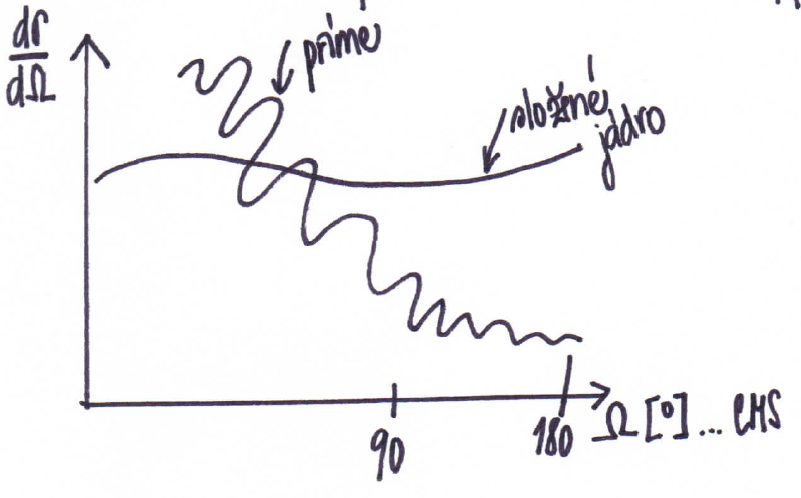
\includegraphics[width=0.6\textwidth]{uhl.png}
	\captionof{figure}{Srovnání úhlových rozdělení}		
\end{center}

\subsection{Princip detailní rovnováhy}

Nízkoenergetické reakce $\rightarrow$ energie interakce $H_{int}$ $<<$ energie celé soustavy $\rightarrow$ lze pro určení pravděpodobnosti $P_{if}$ přechodu od stavu $\phi _i$ ke stavu $\phi _f$ použít zlaté pravidlo poruchového počtu:
\begin{equation}
P_{if} = \dfrac{2 \pi}{\hbar} |H_{fi}| ^2 \dfrac{d \nu}{dE_0},
\end{equation}
kde $H_{fi}$ je maticový element přechodu: $H_{fi} = <\phi _f | H_{int} | \phi _i> = \int \phi^{*}_f
H_{int} \phi_i dV$

V objemu $V$ je počet $d \nu$ stavů (elementárních buněk po jedné částici s hybností $p\div p + dp$):
\begin{equation}
d \nu = \dfrac{V \cdotp 4 \pi \cdotp p^2 dp}{h^3} = \dfrac{4\pi \cdotp V p^2 dp}{(2 \pi \hbar ^3)}
\end{equation} 
a tedy:
\begin{equation}
\dfrac{d \nu}{dE_0} = \dfrac{1}{dE_0} \dfrac{4\pi \cdotp V p^2 dp}{(2 \pi \hbar ^3)}
\end{equation}

Dále uvažujme reakci $A(a,b)B$ v těžišťové soustavě. V konečném stavu platí: $\vec{p_b} = - \vec{p_B}$ $\rightarrow$ pouze jedna nezávislá hybnost (zvolme $p_b$). Jestli $dE_0 = dE_b + dE_B$: 
\begin{equation}
\dfrac{d \nu}{dE_0} = \dfrac{1}{dE_b + dE_B} \dfrac{4\pi \cdotp V_b p_{b}^2 dp_b}{(2 \pi \hbar ^3)}
\end{equation}

Dosadíme za $dE = (p/m) dp$:
\begin{equation}
dE_b + dE_B = \dfrac{p_b}{m_b}dp_b + \dfrac{p_B}{m_B}dp_B = \left(\dfrac{1}{m_b} + \dfrac{1}{m_B} \right) p_b dp_b = \dfrac{1}{m_f} p_b dp_b ,
\end{equation}
kde $m_f$ je redukovaná hmotnost konečného stavu.

Pak dostaneme:
\begin{equation}
\dfrac{d \nu}{dE_0} = \dfrac{4\pi \cdotp V}{(2 \pi \hbar ^3)} m_f p_b.
\end{equation}

Má-li částice (fermion) spin $I$, podle Pauliho principu může být v každém stavu $2I + 1$ částic. Platí to pro oba produkty reakce:
\begin{equation}
\dfrac{d \nu}{dE_0} = \dfrac{4\pi \cdotp V}{(2 \pi \hbar ^3)}(2 I_b + 1)(2I_s + 1)m_f p_b
\end{equation}

Dosadíme do výrazu pro pravděpodobnost ($P_{if} = \dfrac{2 \pi}{\hbar} |H_{fi}| ^2 \dfrac{d \nu}{dE_0}$)
\begin{equation}
P_{if} = \dfrac{2 \pi}{\hbar} |H_{if}|^2 \dfrac{4\pi \cdotp V}{(2 \pi \hbar ^3)} (2 I_b + 1)(2 I_B + 1)m_f p_b = |H_{if}|^2 \dfrac{4\pi  \cdotp V}{(2 \pi )^2 \hbar ^4} (2 I_b + 1)(2 I_B + 1)m_f p_b
\end{equation}

Vztah mezi diferenciálním účinným průřezem a pravděpodobností přechodu:
\begin{equation}
\left( \dfrac{d \sigma}{d \Omega}\right)_{\theta} = \dfrac{(P_{if})_{\theta}}{j} = \dfrac{P_{if}}{4 \pi \cdotp j} ,
\end{equation}
kde $(P_{if})_{\theta} = (1/4 \pi)P_{if}$ pravděpodobnost vztažená na jednotku prostorového úhlu. Hustota toku dopadajících částic: $j = N v_i$, kde $v_i$ je rychlost dopadajících částic a $N$ je jejich počet v jednotce objemu. Vztáhneme-li jej na jednu dopadající částici ($V$ je objem zaujímaný jednou částicí):
\begin{equation}
N = 1/V, ~~~~~~ \rightarrow j = v_i /V
\end{equation}

Potom 
\begin{equation}
\left( \dfrac{d \sigma}{d \Omega}\right)_{\theta} = \dfrac{P_{if} V}{4 \pi v_i} = \dfrac{V m_i}{4 \pi \cdotp p_i} P_{if}, 
\end{equation}
kde $m_i$ je redukovaná počáteční hmotnost (jádro považujeme za nehybné, takže $v_i$ je vzájemná rychlost). Dosadíme za $P_{if}$:
\begin{equation}
\left( \dfrac{d \sigma}{d \Omega}\right)_{\theta} = \dfrac{V^2 (2I_b + 1)(2 I_B +1)}{(2 \pi)^2 \hbar^4} |H_{fi}|^2 m_i m_f \dfrac{p_f}{p_i} = \dfrac{(2I_b + 1)(2I_B + 1)}{(2 \pi)^2 \hbar^4} |H_{if}|_{norm} ^{2} m_i m_f \dfrac{p_f}{p_i}  
\end{equation}	

Člen $V^2$ se pokrátil s faktorem $1/V^2$, který se objeví před členem $|H_{if}|$ v případě normování vlnových funkcí členem $1/\sqrt{V}$. Úhlová závislost je plně obsažena v $|H_{fi}|$.

Odvodíme obdobný vztah pro inverzní proces.

Jestliže: $|H_{fi}|^2$ = $|H_{if}|^2$ spočteme poměr obou účinných průřezů:
\begin{equation}
\dfrac{\sigma_{i\rightarrow f}}{\sigma _{f \rightarrow i}}  = \dfrac{(2I_b + 1)(2I_B + 1) p_{f}^{2}}{(2I_a +1)(2I_A + 1) p_{i}^{2}}
\end{equation}

Tento vztah se nazývá princip detailní rovnováhy jaderné reakce.

Je-li v malé oblasti energií $|H_{if}|^2$ konstantní, dostáváme : $\sigma = konst. \dfrac{p_f}{p_i}$	

\subsection{Model složeného jádra}

$\rightarrow$ vhodný pro neutrony s $T_n < 1 ~\mathrm{MeV}$

- v r. 1936 dánský fyzik Niels Bohr $\Rightarrow$ chtěl vysvětlit jaderné reakce jako dvoufázový proces sestávající nejdříve z vytvoření relativně dlouhožijícího přechodového jádra a jeho následného rozpadu

- bombardující částice nejprve ztratí veškerou svou energii v cílovém jádře (po vniknutí do jádra v něm vykoná několik srážek s nukleony, při nichž ztratí tolik energie, že již není schopna jádro opustit), načež se stane nedílnou součástí nového excitovaného nestabilního jádra zvaného složené jádro
\begin{equation}
a+A \rightarrow C^* \rightarrow b+B
\end{equation}

- rozpad složeného jádra: $10^{-19} ~\mathrm{s} - 10^{-15} ~\mathrm{s}$

$\Rightarrow$ jádro přechází do stabilního stavu $\Rightarrow$ emisí kvant $\gamma$, emisí částice (n, p, $\alpha$) $\Rightarrow$ emitovány izotropně do všech směrů (jádro "zapomíná", jakým způsobem vzniklo)

$\Rightarrow$ druhá etapa jaderné reakce je nezávislá  na první

$\Rightarrow$ ztrácí se informace o původní částici

- máme buď reakci:
\begin{itemize}
	\item rezonanční
	\item nerezonanční
\end{itemize}

- představme si, že nalétávající částice $a$ je nukleon $\Rightarrow$ aby se vytvořilo složené (nestabilní) jádro $C^{*}$ $\Rightarrow$ musí se nukleon dostat na nějakou neobsazenou hladinu v tomto jádře $\Rightarrow$ vytvořené jádro je nestabilní

$\Rightarrow$ energetickým hladinám nukleonů v jádře budou obecně příslušet nenulové šířky hladin $\Gamma$, které umožňují zánik daného nestabilního stavu 

$\Rightarrow$ střední doba života nestabilního jádra je $\tau = \dfrac{\hbar}{\Gamma}$

\begin{itemize}
	\item rezonanční charakter
	
	$\rightarrow$ jednotlivé energetické hladiny i s jejich šířkami $\Gamma$ dostatečně daleko od sebe $\Rightarrow$ $\Delta E >> \Gamma \rightarrow \sigma (E)$
	
	$\rightarrow$ dopadající neutron může vytvořit složené jádro jen tehdy, když jeho energie bude ležet v blízkém okolí ostré hodnoty příslušné danému energet. stavu
	
	$\rightarrow$ rezonanční maximum v průběhu účinného průřezu v místě izolované (od ostatních hladin oddělené) hladiny $E_{res}$
	
	$\rightarrow$ tvar rezonance popisuje Breit-Wignerův vzorec:
	\begin{equation}
	\sigma_{cb} = \pi g \left( \dfrac{\lambda _a}{2 \pi}\right)^2 \dfrac{\Gamma _a \Gamma_b}{(E - E_{res})^2 + (\Gamma /2)^2} 
	\end{equation}
	\begin{equation}
	g = \dfrac{2 I_c + 1}{(2 I_a + 1)(2 I_A + 1)}
	\end{equation}
	
- pro oblast okolo 1-20 $\mathrm{MeV}$ rezonance hustě blízko sebe a jsou široké 

- nedají se rozdělit - vzniká kontinuum (statistická oblast)

\item nerezonanční charakter

$\rightarrow$ když budou jednotlivé energetické hladiny složeného jádra ležet velmi blízko u sebe $\Rightarrow$ svými šířkami se budou prakticky "překrývat", neutron o energii ležící v relativně širokém intervalu může vytvořit složené jádro $\Rightarrow$ $\Delta E << \Gamma \rightarrow \sigma(E)$

- účinný průřez: $\sigma_{ab} = \sigma _{ac} \cdotp \sigma _{cb} = \sigma _{Ac} \dfrac{\Gamma_b }{\Gamma}$	

- $\Gamma_b$ je pravděpodobnost, že rozpad $C^{*}$ bude probíhat s vysláním částice $b$ $\Rightarrow$ představuje současně šířku energetické hladiny $C^{*}$
\begin{equation}
\Gamma_b = \dfrac{\hbar}{\tau _b} = \hbar \omega_b  ~~~~... \textit{Heissenbergův princip neurčitosti}
\end{equation}

- $\Gamma$ je celková šířka = součet částečných šířek hladin ( $\Rightarrow$ doba života $\tau$)
\begin{equation}
\Gamma = \Gamma_{\gamma} + \Gamma_a + \Gamma_{a^{'}} + \Gamma_b + ...
\end{equation}

\item možná reprezentace reakce přes složené jádro v rámci kapkového modelu:

- vybuzené složené jádro - ohřátá kapka vody

- snížení energie výletem nukleonů - ochlazení odpařením molekul $\Rightarrow$ vypařovací modely
\end{itemize}

- Maximum pro pružnou část: $\Gamma_b = 0, \Gamma_a = \Gamma$ : $\sigma_{aamax} = 4  \dfrac{\pi}{k_{a}^{2}}$
	
- Maximum pro nepružnou část: $\Gamma_b = \Gamma_a = \Gamma/2$ : $\sigma_{abmax} = \dfrac{\pi}{k_{a}^{2}}$	

\subsection{Přímé jaderné reakce}

\begin{equation}
a + A \rightarrow b + B
\end{equation}

- trvá: $10^{-22} ~\mathrm{s}$ - čas průletu projektilu terčíkem (pružný a nepružný rozptyl)

- částice se srazí s jedním ( nebo s několika) z nukleonů a uvede jej do vyššího energetického stavu nebo jej vyrazí z jádra (uvolní z vazby v poli jaderných sil )

- sama částice může zůstat v jádře vázána, nebo jej opustí

- i případ dvojnásobné kolize, srážka primární částice s 2 nukleony

- přímý proces = při interakci předá dopadající částice nukleonům jádra hybnost přímo

\begin{itemize}
	\item reakce strhávání - z deuteronu může být stržen neutron a pohlcen terčíkovým jádrem, zatímco proton pokračuje v pohybu ve směru pohybu deuteronu $\Rightarrow$ reakce (d,p)
	
	$\Rightarrow$ při vyšších energiích i (d, n) způsobená strháváním protonů
	
	\item reakce vytrhávání (nabírání) - (n,d), (p,d) - vytržení nukleonu z jádra kolem letícím projektilem
	
	\item reakce přenosu (vybíjení) - výměna nukleonů mezi terčíkem a projektilem
\end{itemize}

- Rozdíly ve srovnání s reakcí přes složené jádro:
\begin{itemize}
	\item úhlové rozdělení je nesymetrické - silný vzrůst intenzity ve směru dopadu
	\item excitační funkce nemá rezonanční charakter 
	\item větší podíl vyletujících částic s vyšší energií
	\item relativní poměry účinných průřezů různých procesů neodpovídají modelu složeného jádra 
\end{itemize}	

\subsection{Modely jaderných reakcí}

Pro popis reakcí se vytvářejí modely, které popisují různé třídy reakcí. 

Střední potenciál jádra vytvářený nukleony terčíkového jádra. 

Projektil vletí do jádra $\rightarrow$ je pod vlivem středního potenciálu $\rightarrow$ ten se může změnit vlivem energie projektilu.

Nutnost započítání vlivu elektromagnetické interakce a coulombovské pole - fotojaderné a elektrojaderné reakce, reakce coulombovského  buzení. Elektromagnetickou část interakce lze spočítat přesně. 
 
\begin{itemize}
	\item OPTICKÝ MODEL - jádro je spojité prostředí - láme a pohlcuje de Broglieho vlnu spojenou s nalétávající částicí
	\item STATISTICKÝ MODEL - v reakcích přes složené jádro spousta mezistavů $\rightarrow$ velký počet stupňů volnosti $\rightarrow$ uvažujeme pouze střední hodnoty veličin
	\item KASKÁDNÍ MODELY - vysoké (relativistické) energie $\rightarrow$ malá vlnová délka nukleonů $\rightarrow$ nukleony dobře lokalizovány $\rightarrow$ reakce (tříštivá) jako sekvence srážek jednotlivých nukleonů
	
- jaderná reakce je popsána úplně - známe $\sigma$ pro všechny měřitelné parametry (energie, úhly, druhy částic ...). Tomu se lze blížit v modelech přímých reakcí, nelze v statistickém modelu.	
\end{itemize}

\subsection{Optický model}

Při hrubém průměrování excitační funkce se ukáže i rozdělení vykazující ve směru dopadu maxima vznikající při ohybu $\rightarrow$ potenciálový rozptyl. Kromě potenciálového rozptylu je třeba popsat i pohlcení dopadající částice (vznik složeného jádra).

Lze popsat optickým modelem:

Předpoklad: jádro je spojité prostředí, které láme a absorbuje de Broglieho vlny dopadajících částic.

Limitní případ je model černého tělesa $\rightarrow$ jádro pohlcuje všechny dopadající částice.

Zjednodušení: reakce dopadající částice s jádrem se aproximuje rozptylem a pohlcením částice silovým centrem

Problém $A_1 + A_2$ částic $\rightarrow$ problém dvou částic

Hledá se tvar středního potenciálu (optický potenciál) U(r) vytvářený silovým centrem, který po dosazení do Schr$\ddot{o}$dingerovy rovnice a splnění okrajových podmínek dává přímo střední hodnotu amplitudy rozptylu.

Optický potenciál zavedeme jako empirický potenciál. Volba parametrů $\rightarrow$ spočítání diferenciálního účinného průřezu $\rightarrow$ porovnání s experimentálním úhlovým rozdělením.

Přítomnost absorbce $\rightarrow$ komplexní člen $\rightarrow$ $U(r) = V(r) + i W(r)$

Reálná část $V(r)$ má tvar potenciálu slupkového modelu (nejčastěji Woodsova - Saxonova tvaru se započtením spin-orbitální interakce) 

Imaginární část: nízké energie $\rightarrow$ převaha absorbce na povrchu

vyšší energie ($\geq 80 ~\mathrm{MeV}$) $\rightarrow$ převaha absorbce v objemu

Při konkrétních výpočtech je třeba započítat vliv coulombovského potenciálu a odstředivého potenciálu.

\end{document}